
 %------------------------------------------------------------------------------------------------------------
 % FILE: 			HivmTex.tex
 % AUTHOR:		Ed Johnson
 % DATE:			June, 2005 (starting conversion to LaTeX.
 % PURPOSE:		Final Research Project for Ed Johnson's Masters Degree.
 % PROFESSOR:	Dr. Ljubomir Buturovic
 %------------------------------------------------------------------------------------------------------------
 
 \documentclass[12pt]{report}
 
 \renewcommand{\baselinestretch}{2}
 \usepackage{latexsym}
 %\usepackage{epsf}
 \usepackage{psfig}
 \usepackage{sfsuthesis}
 \usepackage{graphicx}
 
 %Set the bottom margin to 1in
 %\addtolength{\topmargin}{+.5in}
 %\addtolength{\textheight}{.5in}
 
 \tablespagefalse
 
 \begin{document}
 \title{HIVM - An Application for Prediction of HIV Drug Resistance using Support Vector Machine Algorithms}
 \author{Ed Johnson}
 \submitdate{June, 2005}
 
\beforepreface
\prefacesection{Abstract}
Drug resistance is arguably the most important topic in HIV treatment today.  Current laboratory methods for determining drug resistance have many shortcomings such as high cost, long waits for results, and inability to predict resistance in many circumstances. Our application for predicting drug resistance, hivm, overcomes these obstacles by using a classification algorithm known as Support Vector Machine (SVM). We map HIV amino acid sequences with known drug resistance values to an SVM compatible format that allows us to train and predict drug resistance.   We have conducted a statistical analysis of hivm's ability to predict based on genotypic and phenotypic datasets. Unfortunately, the results show fair to poor prediction of drug resistance for HIV strains that were unknown to the training set.  Furthermore, for the application's true effectiveness to be measured, we would need access to patient response datasets from clinical trials. This data is currently unavailable to us.
\afterpreface

%----------------------------
%   CHAPTER : INTRODUCTION
%----------------------------

\chapter{Introduction}
\label{cha:Introduction}


Drug resistance is arguably the most important topic in HIV treatment today.  Once potent HIV suppression is achieved in previously untreated persons through drug therapy, it usually persists indefinitely if therapy is not interrupted. However, innumerable genetically distinct variants (quasispecies) evolve within an individual in the months following primary infection if left untreated. Tens of thousands of individuals who began HIV therapy in the early and mid-1990s already harbor multidrug-resistant viruses. In addition, a significant proportion of new HIV infections result from the transmission of strains that are already resistant to one or more antiretroviral drugs, and the number keeps growing. [1]

The long-term goal of the hivm project is prediction of patient response
to HIV drug therapy given a genotype of the virus found in the
patient. Ultimately, this would lead to a diagnostic test which may
aid a physician in prescribing a most efficient HIV drug regimen for a
particular patient.

The principal resource we will use in this project is the Stanford HIV
Drug Resistance Database [2], developed under
the guidance of Prof. Robert Shafer. It contains a rich collection of
documentation and data related to the problem we are studying. In
particular, the Drug Resistance Notes sections contains crucial
scientific background for the problem of HIV drug resistance.

In order to achieve the goal outlined above, we plan to use machine learning, and in particular a classification algorithm known as 'Support Vector
Machine' (SVM). The idea is to train the learning machine (SVM) using
known patterns of patient drug resistance for various virus
genotypes. The SVM learns the dependency of drug resistance
vs. virus genotype with sufficient accuracy as predicted by
statistical measures developed during the learning process.  Once this is achieved, it can be applied to classifying previously unseen patients (as represented by
their viral genotype signatures) into the response/no-response
categories.


%----------------------------
%   CHAPTER : Biology and Medical Background
%----------------------------

\chapter{Biology and Medical Background}
\label{cha:Biology and Medical Background }
Now, we will review some important biological concepts that are necessary to understand the problem that hivm attempts to solve. 
		
\section{What is drug resistance?}
\label{sec:What is drug resistance?}		

HIV drug resistance refers to a reduction in the ability of a particular drug or combination of drugs to block reproduction or "`replication"' of HIV. For people infected with the virus, drug resistance can render drugs less effective or even completely ineffective, thus significantly reducing treatment options.
Resistance typically occurs as a result of changes-called mutations-in HIV's genetic structure (RNA). Mutations of RNA lead to alterations in certain proteins, most commonly enzymes, that regulate the production of infectious virus. Mutations are especially common in HIV, as this virus reproduces at an extraordinary rate and does not contain the proteins needed to correct mistakes made during copying of the genetic material. HIV relies on many enzymes-such as reverse transcriptase, integrase, and protease-to replicate inside a human cell.  If a mutation of a single site in the reverse transcriptase gene occurs, the change will remain with the virus as long as it replicates or until another copying error alters its form yet again. Some mutations cause the virus to become so weak that it cannot replicate effectively; other mutations may cause the virus to become even more virulent.
Antiretroviral drugs, generally speaking, disrupt the HIV enzyme's ability for genetic copying, or making virus that can infect other cells. In a person who takes antiretroviral drugs, most of the HIV are killed or prevented from multiplying further. As a result of random mutations that occur on a daily basis, however, some strains of HIV are naturally resistant to the presence of such drugs. That is why treatment with monotherapy (a single antiretroviral drug) is destined to fail.[3] 

\section{How is a patient's drug resistance currently determined?}
\label{sec:How is a patient's drug resistance currently determined?}		

HIV drug resistance occurs when the virus is able to resist the drugs ability to suppress or limit its reproduction. There are currently two tests used to measure for drug resistance. One kind of test is called a "genotypic" test, the other is called a "phenotypic" test. Resistance testing can be helpful for people who are just starting on medication and for people who have taken several different medications over a number of years and are experiencing viral rebound. [5]

\section{What is Viral Load?}
\label{sec:What is Viral Load?}

Viral load measures the amount of HIV virus in one milliliter of a patient's blood. The higher the viral load, the faster the HIV disease progresses. The viral load test is a valuable tool to determine if antiviral drugs are controlling the infection. The best tests as of this writing can detect viral loads as low as 5 copies per milliliter, though the original tests bottomed out at 10,000 copies per milliliter. Only 2\% of HIV in a patient's body resides in the blood, so viral load tests cannot determine whether a patient has removed all HIV from their body.  US treatment guidelines suggest that anyone with a viral load over 55,000 should be offered antiviral treatment. [4]

\section{What is a "Genotypic" Test?}
\label{sec:What is a "Genotypic" Test?}

A genotypic test is a test that examines a specific person's HIV to see if the virus has mutations, and to determine where in the genetic structure of the virus those mutations occur. (Hence the name "genotypic".) Any mutations that are identified through this test are then compared with known drug resistant mutation points for all of the currently available HIV drugs. If there is a match between an identified mutation in the specific person's HIV and known drug-resistant mutation points, the virus is believed to be resistant to those drugs where there is a match.


Genotypic testing can be done in people with a viral load under 1,000 because genotypic testing only involves comparing a person's specific HIV mutations to known drug resistant mutation points. The test can be highly predictive of drug resistance for the "nucleoside analog" class of drugs (AZT, 3TC, ddI, etc.) and "non-nucleoside reverse transcriptase inhibitors" (Sustiva, Viramune, etc.) because these classes of drugs have fairly consistent mutation patterns. However, this test is less predictive of resistance patterns for "protease inhibitors" (Crixivan, Fortovase, etc.) since this class of drugs is not always consistent in the pattern of mutations it produces.

Genotypic testing is less expensive and much faster than phenotypic testing. [see next section] Cost ranges from \$300 to \$500 per test, and results are usually available within a week. � The data reported back can be very difficult to understand, even for physicians, so those unfamiliar with how to interpret the test may need to consult with a specialist in HIV care who is familiar with how to read and interpret the results. [5]

\section{What is a "Phenotypic" Test?}
\label{sec:What is a "Phenotypic" Test?}

In a phenotypic test, a person's blood is divided into many test tubes. A different HIV drug is mixed into each test tube. The virus in each tube is then watched to see which drugs it is able to rapidly produce in the presence of. The amount of drug in each test tube is then increased until it is enough to stop virus reproduction. Based on the amount of drug necessary to stop viral reproduction, a resistance "profile" is created. A simplified way to think of the resistance profile for each drug is:

   1. Low-level resistance: when a 2 to 4 fold [2 fold = 200\%] increase in the amount of drug in the test tube is needed to stop HIV reproduction.

   2. Some resistance: when a 4 to 10 fold increase in the amount of drug in the test tube is needed to stop HIV replication.

   3. High-level resistance: when a 10 fold increase or greater in the amount of drug in the test tube is needed to stop HIV replication. 

Drugs which have a "low-level resistance" or "some resistance" may still work for the individual person as a part of combination therapy. Drugs which have a "high-level resistance" profile are believed to be ineffective in suppressing the virus, and increasing the dosage levels is not thought to be effective.

Phenotypic testing is generally most effective when a person's viral load is greater than 1,000. (For this reason, your provider may not do a phenotypic test if you have a viral load less than 1,000.) A downside to this test is that it does not measure how well different drugs work together in combination (and we know that some drugs can both increase or decrease how well other drugs work when used in combination with each other.) Phenotypic testing is very expensive, and costs about \$1,000 each time the test is done. Also, it takes about 4 to 6 weeks to test a specific person's HIV against all the various drugs. As with genotypic testing, the results can be difficult to interpret and your provider may need to consult with an HIV specialist who knows how to read and interpret this test to make specific drug recommendations.[55]  

\section{What gaps does hivm hope to fill?}
\label{sec:What gaps does hivm hope to fill?}

Regarding genotypic testing, the current methods are not good for predicting resistance to the Protease Inhibitor class because "this class of drugs is not always consistent in the pattern of mutations it produces". [3] hivm has been designed for predicting drug resistance of this case.

Regarding phenotypic testing, the current methods are time consuming and expensive. A physician needs to prescribe the first anti-HIV combination before the 4-6 week delay for phenotypic results.  hivm has a much faster and cost effective turnaround. More importantly hivm is predicting resistance, rather than reacting to existing resistance.  During the first 4-6 weeks, a newly diagnosed HIV patient must start treatment. Due to the high mutation rate of HIV, even four weeks of incorrect therapy could have severely detrimental effects for the patient's long term prognosis. On an individual basis, hivm should be iteratively run and validated against phenotypic testing. Hence, patients should be periodically retested to see if their HIV strains are mutating during treatment. Individualized patient treatment that changes and adapts to the rapidly mutating virus could be far more effective than a static one-time assessment of a patient's HIV condition.

In addition, a mutation may mean that a HIV strain does not reproduce as efficiently as the wild type, even when not in the presence of any anti-HIV drugs.  Normally, this strain would not be able to use the body's resources as well as normal HIV, and would quickly be wiped out. However, if an HIV drug is actively preventing the wildtype from reproducing , then one of the reproductively inferior strains may now have the most access to the body's reproductive facilities. If the current drug does not bind well to the mutant strain because the binding site has changed, then though this strain may not grow as fast as the wildtype, it will still increase the infection. It will still destroy the patients immune system, but at a slower rate than the wildtype.

Since HIV strains with similar sequence of amino acids have a similar binding sites for the drug, we may infer a similar binding affinity to a given drug. We use a variation of the  Smith-Waterman algorithm   known as Local Alignment to produce a score that computes the similarity of two amino acid sequences.  The function we are studying is the binding affinity of a drug to an HIV enzyme.  We expect the sequence similarity to be the best predictor of function that we have at our disposal.

  Combinations of drugs from at least two of the four available drug classes are usually required to achieve durable HIV suppression. Thus HIV cross-resistance to multiple drugs significantly limits treatment options. In other words, if a doctor's first attempt to treat an HIV patient uses drugs that the patient already won't respond to, then the chances of the patient suppressing HIV decrease dramatically. However, if the doctor calculates the correct drug combination the first time, then the patient has a great prospect of suppressing HIV indefinitely and living a healthy normal life.  Though this prescription will be the single most important decision in the patient's treatment, physicians currently have very limited resources available to help them make this decision.

While phenotypic and genotypic tests  provide a useful guess as to HIV strain B's resistance to various drugs. The fact is that the human body is a far more complex setting for this reaction to take place, and there are often unexpected results that do not match up directly to the phenotypic and genotypic tests.  Clinical trials are the most useful source of data for drug resistance because they provide inside into true drug resistance behavior in a human body, where it matters.

\section{Limitations in our model vs. the real world biology of the problem.}
\label{sec:Limitations in our model vs. the real world biology of the problem.}


- We are testing with phenotypic and genotypic datasets because we do not yet have access to clinical trial datasets. While hivm can assess whether a drug can stop the growth of HIV in a lab environment, clinical trial patient response results would be the gold standard to see if we can predict resistance in patients.

- We can only produce prediction models based upon one viral genotype's resistance to one drug at a time. In reality, the factors of drug resistance are much more complex. For instance, every single patient is treated with three at least anti HIV drugs at once, and the three drugs come from three different classes of anti HIV drugs. 

In addition, we do not have data of a given viral genotypes resistance in the presence of more than one drug at a time. It is very, very important to predict HIV variants will exhibit complex cross resistance to multiple drugs at once.  "`A major problem with genotypic testing is that it will miss unknown gene mutations. Also, while the effects of some mutations are clear-cut, this is not always true. A mutation that does not cause resistance by itself could lead to resistance when combined with other mutations. Also, resistance to one drug sometimes results in increased sensitivity to another. One example is that resistance to 3TC reduces resistance to AZT."' [7]

Patient response results from clinical trials should help us to overcome these limitations because patient's are normally treated using combination therapy. Therefore, we would train hivm on the results of combination therapy, and our training model would contain information about cross resistance and other factors that may not have been quantified in a lab setting.


%----------------------------
%   CHAPTER : Support Vector Machines 
%----------------------------

\chapter{Support Vector Machines }
\label{cha:Support Vector Machines }
Our software application uses Machine Learning, specifically a class of statistical algorithms known as Support Vector Machines (SVM) published by Dr. Vladimir Vapnik. [8] SVM's are "`learning systems that use a hypothesis space of linear functions in a high dimensional feature space, trained with a learning algorithm from optimization theory that implements a learning bias derived from statistical learning theory."' 

There are many advantages inherit in SVM's. SVM can classify large data sets of several thousand points while making very, efficient use computer memory.  They can predict previously unseen data well (generalization) by avoiding overfitting to training data.  They have a fast training time compared to competing learning methods such as neural networks.  They have already been used successfully in homology detection of proteins. In addition, "`the set of approximating functions used in the support vector machine ensures that complexity is controlled independently of the dimensionality of the feature space.  Hence, SMV can use large (infinite) dimensional feature spaces."' [9]  This permits the application to accept very large datasets without increasing computational time linearly as more variables are added. 

Additionally, one of the most appealing features of kernel algorithms is the solid foundation provided by both statistical learning theory and functional analysis. Kernel methods let us interpret (and design) learning algorithms geometrically in feature spaces nonlinearly related to the input space, and combine statistics and geometry in a promising way. Kernels provide an elegant framework for studying three fundamental issues of machine learning.

\section{Three fundamental issues of machine learning}
\label{sec:Three fundamental issues of machine learning}

- \textit{Similarity measures} -the kernel can be viewed as a (nonlinear) similarity measure,
and should ideally incorporate prior knowledge about the problem at hand

- \textit{Data representation} - as described above, kernels induce representations of the
data in a linear space

- \textit{Function class} - due to the represented theorem, the kernel implicitly also determines the function class which is used for learning. Support vector machines have been one of the major kernel methods for data classification.[10]

Unlike conventional statistical and neural network methods, the SVM approach does not attempt to control model complexity by keeping the number of features small. Instead, with SVM the dimensionality of z-space can be very large (infinite) because the model complexity is controlled independently of dimensionality.  The motivation for using the high-dimensional feature space is that linear decision boundaries constructed in the high-dimensional feature space correspond to the nonlinear decision boundaries in the input space.  

\section{Two problems overcome by support vector machine in its design}
\label{sec:Two problems overcome by support vector machine in its design}

The conceptual problem is how to control the complexity of the set of approximating functions in a high dimensional space in order to provide good generalization ability.  This problem is solved by using penalized linear estimators with a large number of basis functions.  As shown later in this chapter, the SVM approach results in a constrained quadratic optimization formulation of the learning problem.  

The computational problem is how to perform numerical optimization (i.e. solve quadratic optimization problem) in a high  dimensional space.  This problem is solved by taking advantage of the dual kernel representation of linear functions.  
Kernel functions = inner products in some feature
space (potentially very complex)
 
\section{SVM Background Definitions}
\label{sec:SVM Background Definitions}

\textit{Hilbert space}: Hilbert Space is a vector space H with an inner product $\left\langle{f,y}\right\rangle$  such that the norm defined by
$\left|{f}\right|$ = $\sqrt{\left\langle{f,f}\right\rangle}$
turns H into a complete metric space. If the metric defined by the norm is not complete, then H is instead known as an inner product space. [12]
 
\textit{VC dimension}: size of largest subset of X shattered by
H (every dichotomy implemented) [11]

Bold lower case letters denote vectors

\textit{Structural Risk Minimization}: Minimization of a bound on generalization error

\section{The four distinct concepts of SVM}
\label{sec:The four distinct concepts of SVM} [9]

1. New implementation of the Structural Risk Minimization  inductive principle. Instead of the usual SRM strategy for minimizing the guaranteed risk by minimizing the empirical risk on each element of a structure, the SVM implementation uses a special structure that keeps the value of the empirical risk fixed for all approximating functions but minimizes the confidence interval (for classification problems).

2. Input samples mapped onto a very high-dimensional space using a set of nonlinear basis functions defined a priori.  It is common in pattern recognition applications to map the input vectors into a set of new variables (features) which are selected according to a priori assumptions about the learning problem.  Theses features, rather than the original inputs, are then used by the learning algorithm.  This type of feature selection often has the additional goal of controlling complexity for approximation schemes where complexity is dependent on input dimensionality.  Feature selection capitalizes on redundancy in the data in order to reduce the problem's complexity.  This is in sharp contrast to the approach taken in the SVM which puts no restriction on the number of basis functions (features) used to construct a high dimensional mapping of the input variables.  For the support vector machine, complexity is controlled independently of the dimensionality of the feature space (z-space).

3. Linear functions with constraints on complexity used to approximate or discriminate the input samples in the high-dimensional space.  The support vector machine uses linear estimators to perform approximation.  Many other learning approaches, such as neural networks, depend on nonlinear approximations directly in the samples space.  Nonlinear estimators potentially can provide a more compact representation of the approximation functions; however, they suffer from two serious drawbacks: lack of complexity measures and lack of optimization approaches which provide a globally optimal solution.   Accurate estimates for model complexity can be obtained for linear estimators.  Optimization approaches exist that provide the  (global) minimum empirical risk for linear functions.  For these reasons the support vector machine uses linear estimation in the high-dimensional feature space.

4. Duality theory of optimization used to make estimation of model parameters in a high dimensional feature space computationally tractable.  In optimization theory an optimization problem has a dual form if the cost and constraint functions are strictly convex.  Solving the dual problem is equivalent to solving the original (or the primal) problem [18]. For the SVM, a quadratic optimization problem must be solved to determine the parameters of a linear basis function expansion (i.e., dictionary representation). For high-dimensional feature spaces, the large number of parameters makes this problem intractable.  However, in its dual form this problem is practical to solve, since it scales in size with the number of training samples.  The linear approximating function corresponding to the solution of the dual is given in the kernel representation rather than in the typical basis function representation.  The solution in the kernel representation is written as a weighted sum of the support vectors.  The support vectors are a subset of the training data corresponding to the solution of the learning problem.  The weights have an equivalent representation in the high-dimensional feature space. [9]

\section{Historical Development of SVM}
\label{sec:Historical Development of SVM} 

Optimal Separating Hyperplane
The conceptual problem of how to control the complexity of the set of approximating functions in a high dimensional space in order to provide good generalization ability is solved by use of the 
Optimal Separating Hyperplane.

A separating hyperplane is a linear function that is capable of separating the training data without error.  Suppose that the training data consisting of n samples
 $(\textbf{x}_{1},y_{1}),...,(\textbf{x}_{n},y_{n}), \textbf{x}\in\Re^{d}, y\in\left\{+1,-1\right\}$ can be separated by the hyperplane decision function

\begin{center}
$D(\textbf{x}) = (\textbf{w}\cdot\textbf{x}) + w_{0}$		
\end{center}
		
\begin{flushright}
(3.1)
\end{flushright}

with appropriate coefficeints $\textbf{w}$ and $w_{0}$.  The assumption about linearly separable data will later be relaxed; however, it allows a clear explanation of the SVM approach.  A separating hyperplane satisfies the constraints that define the separation of the data samples: 

\begin{center}
$(\textbf{w}\cdot\textbf{x}_{i}) + w_{0} \geq$ +1 if $y_{i}$ = +1
$(\textbf{w}\cdot\textbf{x}_{i}) + w_{0} \leq$ +1 if $y_{i}$ = -1, i=1,...,n	
\end{center}
	
\begin{flushright}
(9.2)
\end{flushright}

Suppose that the training data consisting of n samples $(\textbf{x}_{1},y_{1}), �,(\textbf{x}_{n},y_{n}), \textbf{x}\in\Re^{d}, y\in\left\{+1,-1\right\}$ can be separated by the hyperplane decision function 
\begin{center}
$D(\textbf{x}) = (\textbf{w}\cdot\textbf{x}) + w_{0}$
\end{center}
A separating hyperplane satisfies the constraints that define the separation of the data samples:
 
\begin{center}
$y_{i}[(\textbf{w}\cdot\textbf{x}_{i}) + w_{0}]\geq$1,i = 1,...,n		
\end{center}
\begin{flushright}
(9.3)
\end{flushright}
 
For a given training data set, all possible separating hyperplanes can be represented in this form (3.3).  This is an important observation, since it allows separating hyperplanes to be described directly in terms of the training data.  The formulation of the separating hyperplane allows us to solve the classification problem directly.  It does not require estimation of density as an intermediate step.  

\begin{figure}
	\centering
		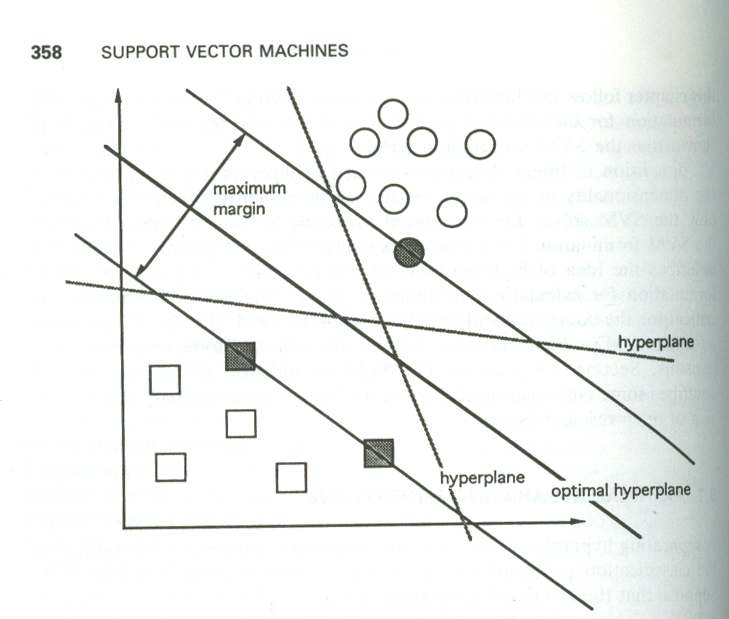
\includegraphics[width=1.00\textwidth]{images/hyperplane1.png}
	\caption{ Separating hyperplanes in a two-dimensional space. An optimal hyperplane is one with a maximal margin. The data points at the margin (indicated in gray) are called the support vectors because they define the optimal hyperplane.}
	\label{fig:hyperplane1}
\end{figure}

The minimal distance from the separating hyperplane to the closest data point is called the margin and will be denoted by $\tau$ . A separating hyperplane is called optimal if the margin is the maximum size . It is intuitively clear that a larger margin corresponds to better generalization.  The SVM framework presented below shows how to formally describe an optimal hyperplane and how to determine it from the training data.  The distance between the separating hyperplane and a sample \textbf{x}' is $\left|D(\textbf{x}')\right|/\left\|\textbf{w}\right\|$, as show in the (fig 3.2)  Assuming that a margin $\tau$ exists, all training patterns obey the inequality:

\begin{center}
$\frac{y_{k}D\left(\textbf{x}_{k}\right)}{\left\|\textbf{w}\right\|}\geq\tau$, k=1,...,n 
\end{center}
			

\begin{flushright}
(3.4)
\end{flushright}

where $y_{k} \in \left\{-1,1\right\}$.	


The problem of finding the optimal hyperplane is that of finding the \textbf{w} that maximizes the margin $\tau$.  Note that there are an infinite number of solutions that differ only in scaling of \textbf{w}. To limit solutions, fix the scale on the product of $\tau$ and norm of \textbf{w}, 
\begin{center}
$\tau\left\|\textbf{w}\right\|=1$
\end{center}

\begin{figure}
	\centering
		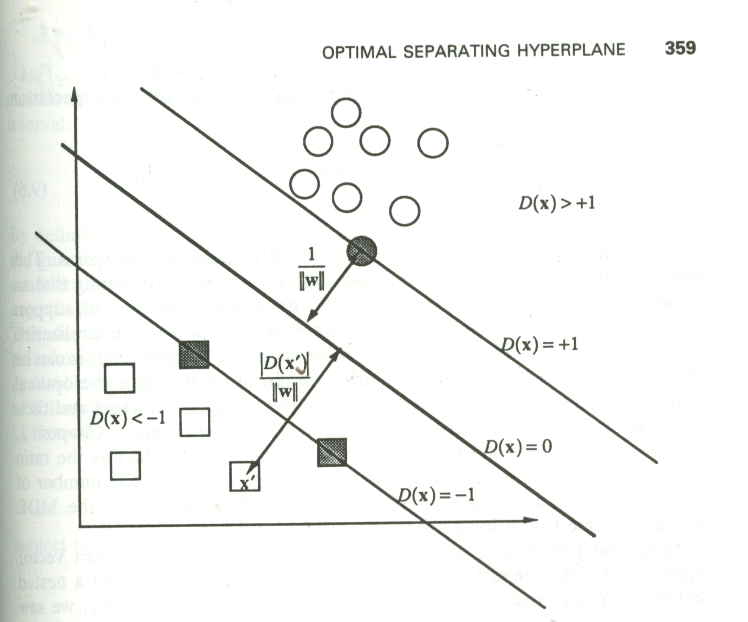
\includegraphics[width=1.00\textwidth]{images/hyperplane2.png}
	\caption{The decision boundary of the optimal hyperplane is defined by points x for which D(\textbf{x})=0. The distance between a hyperplane and any sample \textbf{x}' is  $\left|D\left\langle \textbf{x}'\right\rangle\right| / \left\|\textbf{w}\right\|$.  The distance between a support vector (which defines the margin) and the optimal hyperlane is 1/$\left\|\textbf{w}\right\|$}
	\label{fig:hyperplane2}
\end{figure}


Thus maximizing the margin $\tau$ is equivalent to the minimizing the norm of \textbf{w}.  An optimal separating hyperplane is one that satisfies condition (3.3) above and additionally minimizes

\begin{center}
$\eta(\textbf{w})=\left\|{\textbf{w}}\right\|^{2}$	
\end{center}
	\begin{flushright}(3.5)\end{flushright}

with respect to both \textbf{w} and $w_{0}$.  The margin relates directly to the generalization ability of the separating hyperplane.  The larger the margin, the more separation occurs between the classes.  The data points that exist at the margin, or equivalently, the data points for which (3.3) is an equality are called the \textit{support vectors} (fig 3.2). Since the support vectors are data points closest to the decision surface, conceptually they are the samples that are the most difficult to classify and therefore define the location of the decision surface.  It is shown later that the decision surface of the optimal hyperplane is written in terms of the support vectors.
	The generalization ability of the optimal separating hyperplane can be directly related to the number of support vectors.  According to Vapnik [17] the number of support vectors provides a bound on the expectation of the error rate for a test sample.

\begin{center}
$E_{n}\left[ Error  rate \right] \leq \frac{E_{n}[ Number of support  vectors ]}{\textit{n}}$
\end{center}
 
\begin{flushright}
(3.6)
\end{flushright}

The operator $E_{n}$ denotes expectation over all training sets of size \textit{n}. 
This  bound is independent of the dimensionality of the space. Assuming 
that an optimal hyperplane can be constructed with a small number of 
support vectors (relative to the training set size), it will have good 
generalization ability e\textit{ven in high-dimensional space.}

For the hyperplane functions (3.3) satisfying the constraint ${\left\|\textbf{w}\right\|}^{2}\leq c$ , the VC-dimension is bounded by 
\begin{center}
$\textit{h} \leq min( r^{2} c, d) + 1$			
\end{center}
\begin{flushright}
 (3.7)
\end{flushright}
 where r is the radius of the smallest sphere that contains the training input vectors $(\textbf{x}_{1},...,\textbf{x}_{n}.$

	The factor r provides a scale (in terms of the training data) for c. Notice that it is possible to directly control the complexity of the hyperplane (i.e., the VC-dimension) \textit{independent of dimensionality of the sample space}.   With this measure of the VC-dimension, it is now possible to construct a structure on the set of hyperplanes according to increasing complexity by controlling the norm of the weights $\left\|{\textbf{w}}\right\|^{2}$:
	
\begin{center}
$S_{k} = \left\{ \left(\textbf{w}\cdot\textbf{x}\right) + w_{0}: \left\|{\textbf{w}}\right\|^{2} \leq c_{k} \right\}, c1<c2<c3... $			(3.8)
\end{center}

\section{High-Dimensional mapping and Inner Product Kernels}
\label{sec:High-Dimensional mapping and Inner Product Kernels} 

In the last section, it was shown that optimal hyperplanes are good approximation functions because their complexity can be carefully controlled independent of dimensionality.  Therefore, they are capable of providing good generalization ability even for high dimensions. It was shown how to pose the optimization problem of finding the optimal hyperplanes in a manner that allows practical solution even for high dimensional input spaces.   However,  hyperplanes were only described as linear functions in the \textbf{x}-space.  Now, we will describe how to efficiently construct high dimensional sets of basis functions and then determine optimal hyperplanes in this space.  This high dimensional space is called the feature space in order to distinguish it from the input space (\textbf{x}-space).  
Notice that the optimization problems require the calculation of the inner product between vectors in the \textbf{x}-space, and that this is the only operation requiring the \textbf{x}-values of the training data.  If a large set of basis functions is used (i.e., $\textbf{g}_{j}(\textbf{x}), j=1,...,m)$, then solving the optimization problems would require determining inner products in the feature space defined by the basis functions.   In this section, the set of basis functions is first formally defined, and then the procedure used to compute the inner product of the basis functions is described.  The computation of the inner product corresponds to evaluating an inner product kernel.  Finally, the inner product kernels for a number of common types of basis functions are described.  

	Let us denote $\textbf{g}_{m}(\textbf{x}), j=1..m$, as a set of nonlinear transformation functions defined a priori.  These functions map the vector x into an m-dimensional feature space.  hyperplanes can then be created in this feature space rather than in the input space.   For example, the functions $g_{j}(x), j=1...m$, could correspond to polynomial terms of the components of \textbf{x} up to a certain order (including interation terms). Linear decision boundaries in the feature space would then map to polynomial decision boundaries in the input space. The decision function (3.1) becomes 
\begin{center}
$D(\textbf{x}) =  \sum\limits_{j=1}^{m} w_{j}\textbf{g}_{j}(\textbf{x})$  						(3.9)
\end{center}

where the number of terms in the summation depends on the dimensionality of the feature space.   In the dual form this decision function is
\begin{center}
\[
D(\textbf{x}) =  \sum\limits_{i=1}^{n} \alpha_{i}y_{i}H(\textbf{x}_{i},\textbf{x})		(3.10)
\]
\end{center}

 The \textit{inner product} kernel H is a representation of the basis functions $\textbf{g}_{j}(\textbf{x}), j=1,...,m$.  It differs from the equivalent kernel representation, since it does not incorporate the parameters estimated from the training data. 
The \textit{equivalent} kernel representation \textit{is determined after} the approximating function is found, while the inner product kernel \textit{is known a priori }and used to form a set of approximating functions.   For a given set of basis functions $\textbf{g}_{j}(\textbf{x})$, the inner product kernel H is determined by the sum
\begin{center}
\[
H(\textbf{x},\textbf{x}^{'}) =  \sum\limits_{j=1}^{m} g_{j}(\textbf{x})g_{j}(\textbf{x}^{'})
\]
\end{center}
\begin{flushright}
(9.11)
\end{flushright}

where m may be infinite.
	Notice that in the form (3.11), the evaluation of the inner products between the feature vectors in a high dimensional \textit{feature space} is done indirectly via the evaluation of the kernel H between support vectors in the \textit{input space}.  This solves the technical problem of evaluating inner products in a high dimensional feature space.    The general expression for an inner products in Hilbert space is
\begin{center}
	\[
	(\textbf{z} \cdot \textbf{z}^{'}) = H(\textbf{x},\textbf{x}^{'})
\]
\end{center}
(3.12)

where the vectors \textbf{z} and \textbf{z}' are the image in the m-dimensional feature space and vectors \textbf{x} and \textbf{x}' are in the input space.  
 
	The expansion of the inner product (3.11), (3.12) in the dual representation allows the construction of decision functions that are nonlinear in input space. It also makes computationally possible the creation of a very high dimensional feature spaces, since they do not require direct manipulation. Common classes of basis functions used for learning machines correspond to different choices of kernel functions for computing the inner product.  Below are several common classes of multivariate approximating functions and their inner product kernels:

Polynomials of degree q have inner product kernel:

\begin{center}
	\[
	 H(\textbf{x},\textbf{x}^{'}) = \left[ (\textbf{x},\textbf{x}^{'}) + 1 \right]^{q}
\]
\end{center}
\begin{flushright}
(3.14)
\end{flushright}

\textbf{Radial basis functions} of form:
\begin{center}
	\[
	\textbf{f}(x) = \sin(  \sum\limits_{i=1}^{n} \alpha_{i}\exp\left\{ - \frac{\left|\textbf{x}-\textbf{x}_{i}\right|^{2}}{\sigma^{2}}\right\} )
\]
\end{center}
\begin{flushright}
(3.15)
\end{flushright}

where $\sigma$ defines the width of the inner product kernel
\begin{center}
	\[
	 H(\textbf{x},\textbf{x}^{'}) = \exp\left\{ - \frac{\left|\textbf{x}-\textbf{x}_{i}\right|^{2}}{\sigma^{2}}\right\} )
\]
\end{center}
\begin{flushright}
(3.16)
\end{flushright}

Note that the number of basis functions, the center parameters, that correspond to the support vectors and the weights in the output layer are all automatically determined via the optimal hyperplane.  All basis functions have the same width parameter which is specified a priori.

\section{Support Vector Machine for Classification}
\label{sec:Support Vector Machine for Classification} 

The support vector machine for classification is constructed by applying the concepts of the previous two sections.  The inner product kernel is used to define a high dimensional mapping, and an optimal hyperplane is found in this space.  This corresponds to replacing the inner products in the optimization problems of sections 3.5 with the inner product kernels given in Sections 3.6. First, we will present the final optimization problem statement.  
	
For classification of no separable data, the decision function is given by

\begin{center}
	\[
	D(\textbf{x}) =  \sum\limits_{i=1}^{n} \alpha_{i}^{*}y_{i}H(\textbf{x},\textbf{x}^{'})
\]
\end{center}
\begin{flushright}
(3.17)
\end{flushright}

note that we have dropped the zero-order "threshold" term, since it can be represented by including a constant basis function (ie., \textbf{g}(\textbf{x}) =1 ) in the feature space.  the parameters $\alpha_{i}^{*}$, i=1...n, is the solution for the following quadratic optimization problem:

Maximize the functional

\begin{center}
	\[
	Q(\alpha) = \sum\limits_{i=1}^{n} \alpha_{i} - \frac{1}{2}\sum\limits_{i,j=1}^{n}\alpha_{i}\alpha_{j} y_{i}y_{j}H(\textbf{x},\textbf{x}^{'})
\]
\end{center}
\begin{flushright}
(3.18)
\end{flushright}


subject to constraints

\begin{center}
	\[
	\sum\limits_{i=1}^{n} y_{i}\alpha_{i} = 0, 0\leq\alpha_{i}\leq\frac{C}{n}, i = 1,...,n
\]
\end{center}
\begin{flushright}
(3.19)
\end{flushright}

given the training data $(\textbf{x}_{i},y_{i})$, i=1...,n, an inner product kernel H, and regularization parameter C. At present, there is no well-developed theory on how best to select C. In the applications published to date, it is set to a large fixed constant. For the separable case, C = $\infty$.


	In order to apply the SVM to practical problems, one needs to choose the type of kernel function and the value of C. Rigorous selection of these parameters requires an estimate of the complexity (VC-dimension) and the application of the generalization bound.  Using the generalization bound requires selections for the constants in the bound appropriate for the SVM.  However, "good" values of these constants are not known for SVM and there is no accurate estimate for VC-dimension. Therefore, in practice, resampling techniques are used to choose the type of kernel and the value of C.
[9]  This technique was used in our implementation to find optimal SVM parameters, and will be discussed in greater detail in the next section. 

%----------------------------
%   CHAPTER : Implementation
%----------------------------

\chapter{Implementation}
\label{cha:Implementation}

We have designed and produced a cross platform ANSI C/C++ command line implementation of hivm, that is suitable for standalone use or integration into a larger application. We have placed it under the The MIT License[13]  to make it free for both commercial and non-commercial use. I will discuss some of the problems we overcame developing hivm, and also give more descriptions of the application itself.

\section{Local Alignment}
\label{sec:Local Alignment}

An amino acid sequence folds into a particular structure in a process known as translation. 
This structure determines the functionality of the protein that was based on the amino acid sequence.  In the case of hivm, we are studying two well understood strings of amino acids on HIV. These strings encode two particular enzymes that are
essential to the reproductive cycle of HIV, Reverse Transcriptase and Protease.

These enzymes normally bind with particular molecules in the human body in order to reproduce more HIV. The goal of most HIV anti-viral drugs
is to have the drug molecules bind to these HIV enzymes instead of the molecules that HIV would normally to bind to.  The drug molecules bind to the 
active site of the enzymes, and as long as they are attached to the active site, the cycle of HIV reproduction has been broken.

The most frequently found strain of HIV was used to create modern anti-viral drugs. The drugs are molecules that are known to bind very well to these two active sites. The active sites have a particular three dimensional structure that was determined by the amino acid sequence that encoded them. The drugs also have a site on them that was chosen because it binds very well to one of the two 3D structures at the active sites.

As long as the 3D structure of the active sites remains unchanged, the currently known drugs will do a great job of binding to them and stopping the growth of the HIV infection.  Unfortunately, HIV mutates frequently, and the amino acid sequences for the RT and PI enzymes frequently change.  These mutations are changes in the amino acid sequences that frequently lead to a change in the 3D structure of the active site. This changes the quality of the expected bond between the drugs and HIV enzymes.  Sometimes the drug binds less well to the enzyme, but the enzyme can still bind to the native molecules that it needs for reproduction.  In this case, the HIV infection may have slower growth, but it will still grow. Adding increasing amounts of a particular drug to a patient's system will usually stop the infection, but this increased dosage may cause undesirable and/or toxic side effects in the patient.

Because sequence similarity is usually tightly bound to functional similarity, it is useful to have a method to rate similarity between two amino acid sequences. If we know the drug resistance level of a mutated amino acid sequence, then there is a very good chance that a similar amino acid sequence will exhibit the same drug resistance pattern. Remember that the drug resistance is determined by the structure of the HIV enzymes' active binding sites. 

One of the best methods for determining sequence similarity is called "`the local alignment score"' of two sequences.  This is based on the Smith-Waterman algorithm [6], and it is the method used in hivm. Ljubomir Buturovic wrote the code to compute the local alignment scores needed by hivm to solve the following problem.

SVM requires input data to be a set of vectors where each vector is the same length. Since our mutated list of amino acid sequences are of different lengths, we had to find a way to prepare the data to that it could be used in an SVM.  Buturovic's solution was to take a group of \textit{n} sequences and compare each sequence to every other sequence in the group by using the local alignment function. After this step, each sequence is represented as a vector of local alignment scores.  This produces an n x n matrix of local alignment scores where each vector is now the same length. This took care of the problem of preprocessing the sequences for use by the SVM. 

In practice, alternative methods of sequence comparison could be used by hivm. Local alignment is probably the most well known algorithm for computing sequence similarity in bioinformatics, but there are other methods that could be experimented with in the future.  hivm uses several phases of data processing. In some phases, it is possible to accommodate competing methods to improve accuracy and performance, and encourage further exploration of the problem. 

\section{Issues with Cross-Validation}
\label{sec:Issues with Cross-Validation}

Originally, we used the Libsvm cross validation which worked as follows:
(To keep it simple, let's say we are dealing with 10 total sequences and 10 fold cross validation)

Take a group of sequences from the dataset file. Compute the pairwise alignment (Local Alignment matrix) of all of them, and feed this matrix into the libsvm cross-validation function. Each vector maps back to a sequence from the original dataset. Each sequence also has a resistance category associated with it. (the simplest case is 0/1. resistant or not). This category threshold(s) is selected by the application's user every time he runs the program.

During one iteration of a 10-fold cross validation, 10\% of the local alignment vectors are randomly selected and logically separated from the remaining 90\% of the local alignment vectors. The 90\% of local alignment vectors and their known category value are used to compute an SVM training model. This model is then used to predict the class of the 10\% of local alignment vector's one at a time. Each of the 10\% vector's "`know's"' what category it was originally placed in by the user of the application. The cross validation function compares the known value to the predicted value and stores this statistic for each vector in the 10\% group.

Originally, our prediction functions worked as follows:

A new sequence to be predicted is read into the application from file. This sequence is mapped to feature space by computing it's local alignment value against every sequence that composes the local alignment matrix. This is the local alignment matrix which will be turned into a training model by libsvm. The new sequence's identity local alignment value is dropped, which makes the new sequence's vector of local alignment values the same length as every vector that created the training model.

For our test purposes, we already know which category the new sequence belongs to. We run the libsvm prediction function on the new sequence (which is in local alignment vector form). This produces a prediction of which category the sequence belongs to. We check to see if this is correct or not during testing.

There is one main difference between a single iteration of the cross validation technique and running a prediction.

In cross validation, the training model contains local alignment value(s) that were created by comparing the model's sequence(s) against the sequence(s) to be predicted. In addition, the sequence to be predicted has it's identity local alignment value in it's vector.

In a normal prediction, the training model does not contain any local alignment values computed against the sequence to be predicted. In addition, the sequence to be predicted does not contain it's identity local alignment value. 

 Our SVM library was provided by the Libsvm [15]  project to perform SVM training, cross-validation, and prediction. The amino acid sequences from the Stanford HIV Database project are of different lengths. Since SVM requires input of identical length, we had perform a pair-wise local alignment comparison of each sequence against all other sequences. In this way, we mapped the original input data into an appropriate feature space for by SVM.  Also, because of our special function to map to feature space, we had to write out own cross-validation function.  The Libsvm cross-validation function assumes that each input vector is independent from the others. In our case, each vector contains information about every other vector, and thus the training model would predict a partially known sequence instead of a completely unknown sequence.  In our refactored cross-validation function, we remove all information about the sequence to be predicted from the training model. This ensures that the cross-validation provides honest results.  These two issues will be discussed in the next section in greater detail. 

\section{Libsvm Recommended Procedures}
\label{sec:Libsvm Recommended Procedures}

Libsvm usage is not simple and there are many common pitfalls that new users encounter.  The Libsvm team attempted to rectify this by creatinng a new users guide. There are many procedures recommended by the creators of Libsvm. [15]

� \textit{Transform data to the format of an SVM software}:\newline
(described above in the Local Alignment section)

� \textit{Conduct simple scaling on the data}:\newline
The main advantage is to avoid attributes in greater numeric ranges dominate
those in smaller numeric ranges. Another advantage is to avoid numerical difficulties
during the calculation.


� \textit{Consider the RBF kernel} $K(x, y) = e^{-\gamma\left\|x-y\right\|^{2}}$:\newline
They suggest that in general RBF is a reasonable first choice. The RBF kernel nonlinearly
maps samples into a higher dimensional space, so it, unlike the linear kernel,
can handle the case when the relation between class labels and attributes is nonlinear.
Furthermore, the linear kernel is a special case of RBF as (Keerthi and Lin 2003)[19]
shows that the linear kernel with a penalty parameter C has the same performance as
the RBF kernel with some parameters (C, $\gamma$). In addition, the sigmoid kernel behaves like RBF for certain parameters (Lin and Lin 2003). [20]
The second reason is the number of hyperparameters which influences the complexity
of model selection. The polynomial kernel has more hyperparameters than
the RBF kernel.
Finally, the RBF kernel has less numerical difficulties. One key point is
 0 < \[K_{ij} \leq 1 \] in contrast to polynomial kernels of which kernel values may go to infinity
	\[(\gamma x_{i}^{T}x_{j} + r > 1) or zero (\gamma x_{i}^{T}x_{j} + r < 1) 
\]
while the degree is large. Moreover, they note that the sigmoid kernel is not valid (i.e. not the inner product of two vectors) under some parameters. [17]

� \textit{Use cross-validation to find the best parameter C and $\gamma$ }\newline

There are two parameters while using RBF kernels: C and $\gamma$. It is not known beforehand which C and $\gamma$ are the best for one problem; consequently some kind
of model selection (parameter search) must be done. \newline
They recommend a �grid-search� on C and using cross-validation. Basically pairs
of (C, $\gamma$) are tried and the one with the best cross-validation accuracy is picked. They found that trying exponentially growing sequences of C and $\gamma$ is a practical method to identify good parameters. 

 We used:
	 $ C = 2^{-30}, 2^{-29}, . . . ,2^{29}, 2^{30} $ 
 
 $ \gamma = 2^{-30}, 2^{-29}, . . . ,2^{29}, 2^{30}$


We then used the best penalty parameter C and width parameter gamma to train the whole training set. However, we found a need to use a more advanced analysis of the 'best' cost and gamma parameters that was not described in the Libsvm materials.  We chose a technique known as ROC analysis (Receiver Operating Characteristic).

\section{ROC Analysis}
\label{sec:ROC Analysis}


The area under a ROC curve (AUC) is commonly used as a summary measure of diagnostic accuracy. It can take values from 0.0 to 1.0. The AUC can be interpreted as the probability that a randomly selected diseased case (or "event") will be regarded with greater suspicion (in terms of its rating or continuous measurement) than a randomly selected nondiseased case (or "non-event"). So, for example, in a study involving rating data, an AUC of 0.84 implies that there is an 84\% likelihood that a randomly selected diseased case will receive a more-suspicious (higher) rating than a randomly selected nondiseased case. Note that an AUC of 0.50 means that the diagnostic accuracy in question is equivalent to that which would be obtained by flipping a coin (i.e., random chance). It is possible but not common to run into AUCs less than 0.50. It is often informative to report a 95\% confidence interval for a single AUC in order to determine whether the lower endpoint is > 0.50 (i.e., whether the diagnostic accuracy in question is, with some certainty, any better than random chance). [14]

A ROC curve allows an HIV expert to choose the trade off points between true positive rate and false positive rate for our SVM machine. In other words, a expert  would choose a point on the graph that was best for her situation. That point would give a cost/gamma pair. Then, the expert would train an SVM model with that cost, gamma pair, and predict the classification of her HIV strains using that newly trained model. 

\begin{figure}
	\centering
		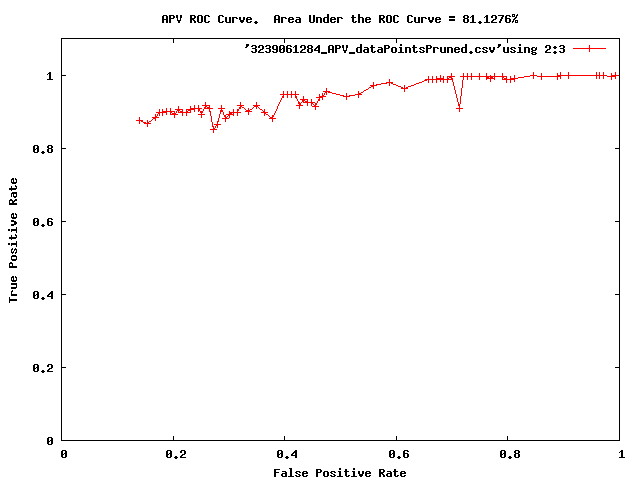
\includegraphics[width=1.00\textwidth]{images/3239061284_APV_.png}
	\caption{The ROC Curve generated by our tests for APV drug. }
	\label{fig:3239061284_APV_}
\end{figure}


\section{Testing}
\label{sec:Testing}

We randomly separated one third of the known sample data to be used as test data. 

\section{Input Data}
\label{sec:Input Data}

The Stanford University HIV Drug Resistance Database group provided the input datasets used for hivm.\newline

The susceptibility methods in the data set below include only ViroLogic$^{TM}$ test results.  The dataset contains 621 Protease (PI)and 418 Reverse Transcripase (RT) sequences from 42 references.


\textbf{Description of Selected Fields in the DataSet Files}\newline
\textit{Field Name}	Description\newline
\textit{SeqID}	Sequence identifier\newline
\textit{Subtype}	Subtype of sequence\newline
\textit{Method}	Phenotype method\newline
\textit{RefID}	Published reference. View References Table\newline
\textit{Type	Clinical vs. Lab Isolate.} Lab isolates are site directed mutants or results of in vitro passage.\newline
\textit{IsolateName}	Isolate identifier\newline
\textit{Drug Fold	}Fold resistance of Drug X compared to the wild type.\newline
\textit{Drug FoldMatch}	Fold match for Drug X. '=' for most results. '$<$' if result is below the lower limit of the assay. '$>$' if the result is greater than the upper limit of the assay.\newline
\textit{P1...P n}	Amino acid at this position. '-' indicates consensus; '.' indicates no sequence; '\#' indicates an insertion; '~' indicates a deletion and a letter indicates one letter Amino Acid substitution.\newline
\textit{Mutation Lists}	Mutation Lists provided at the far right of the output are lists of mutations present in the sequence. Some lists contain all the mutations, others contain specific sublists.\newline


\section{Example of Two Sequences from the PI DataSet}
\label{sec:Example of Two Sequences from the PI DataSet}

 Only a few of the several hundred mutation positions are shown here for space considerations.

\textit	SeqID	SubType	Method		RefID	Type			IsolateName	APV Fold	APV FoldMatch	ATV Fold	ATV FoldMatch\newline
				15526		B			Virologic	824		Clinical	RC-1211.2				3			=		 							5					=\newline
				54306		B			Virologic	1040	Clinical	DD-071049				1			=									na			S	na\newline

\textit{P1	P2	P3...}\newline
I		-		-\newline
-		-		-\newline

\textit{CompMutList}\newline		
L10I, I13V, K20R, E35D, M36I, I54V, L63P, I64V, V82A, L90M\newline
N37C, I54V, I62V, L63P, V82A, I93L\newline

\textit{MajorMutList}\newline
I54V, V82A, L90M\newline
I54V, V82A\newline

\textit{MinorMutList}\newline
L10I, K20R, M36I, L63P\newline
L63P, I93L\newline

\section{Drugs in the Datasets}
\label{sec:Drugs in the Datasets}


{Protease Inhibitor Drugs}\newline
Atazanavir (ATV)\newline
Fosamprenavir (FPV)\newline
Indinavir (IDV)\newline
Lopinavir (LPV)\newline
Nelfinavir (NFV)\newline
Saquinavir (SQV)\newline
\newline
{Reverse Transcriptase AntiViral Drugs}\newline
Abacavir (ABC)\newline
Didanosine (ddI)\newline
Emtricitabine (FTC)\newline
Lamivudine (3TC)\newline
Stavudine (d4T)\newline
Tenofovir (TDF)\newline
Zidovudine (ZDV)\newline
Delavirdine (DLV)\newline
Efavirenz (EFV)\newline
Nevirapine (NVP)\newline

\newpage

\section{Classes}
\label{sec:Classes}

\begin{figure}
	\centering
		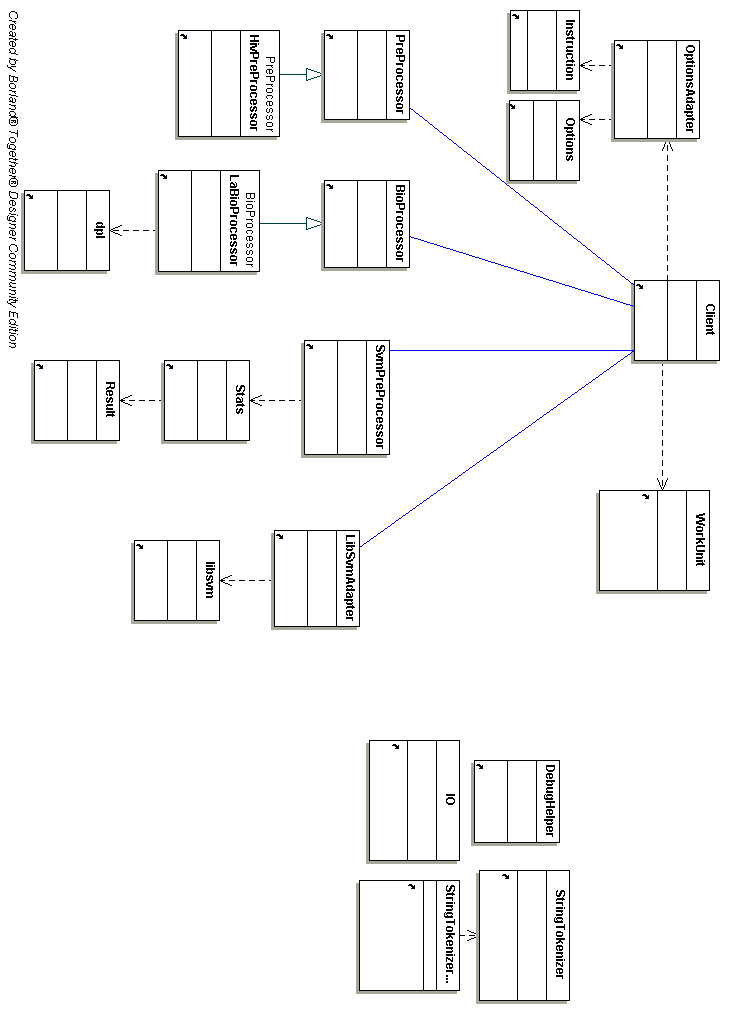
\includegraphics[width=1.00\textwidth]{images/Hivm_uml.png}
	\caption{hivm  UML Diagram}
	\label{fig:Hivm_uml}
\end{figure}

\begin{figure}
	\centering
		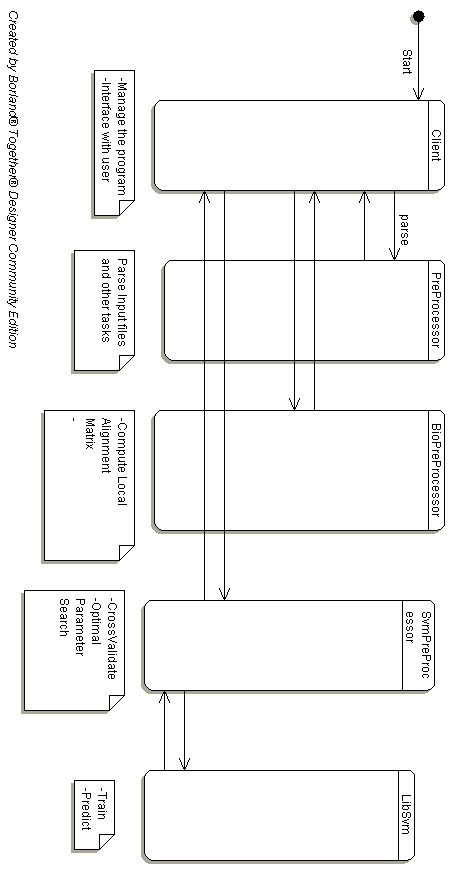
\includegraphics[width=1.00\textwidth]{images/HivmStateChart.png}
	\caption{hivm State Chart}
	\label{fig:HivmStateChart}
\end{figure}


\textit{IO}\newline
purpose save and read files in one in the program
returns true for success, false for failure

\textit{BioProcessor}\newline
@purpose Base class to convert input data from aminio acids to numeric values based upon 
different biological algorithms

\textit{LaBioProcessor}\newline
@purpose Convert input data from aminio acids to numeric values based upon 
local alignment algorithm [6]


\textit{Client}\newline
@purpose Main entry point into hivm. Decides which hivm functionality
to use.

\textit{DebugHelper}\newline
@purpose Static methods to show allow stepping through containers with debugger.

\textit{Hash}\newline
@purpose Hash a string quantity. Used to identify unique results and cached computations on the file system.

\textit{PreProcessor}\newline
@purpose Base class to parse the input files and get them
ready for SVM

\textit{HivPreProcessor}\newline
@purposee Concrete class to parse the Hiv input files and get them
ready for SVM\newline
This version runs the pre November 2004 version of Stanford HIVDB input data sets.

\textit{Instruction}\newline
@purpose: Instruction class is responsible for 
gathering the user instructions from the cmd line,
and providing that data to the rest of the app

\textit{Options}\newline
@purpose Holds libsvm options used in PhaseMachine program

\textit{OptionsAdapter}\newline
@purpose: OptionsAdapter class is responsible for 
gathering the necessary program options from the options text file,
and providing that data to the rest of the app

It provides clean interface to the original PhaseMachine
Options class and the hivm Instruction class which were already created to
hold different sets of options. 

\textit{LibSvmAdapter}\newline
@purpose Provides an interface to the libsvm C-style functions. Provides memory management and error checking using full features of C++. 

\textit{Result}\newline
@purpose Hold results of SVM tests and provide statistics based on them.

\textit{Stats}\newline
@purpose Most basic statistics holder

\textit{WorkUnit}\newline
@purpose: Workunit is designed to hold state of 
data that has been parsed into a SVM compatible 
format by the PreProcessor.

It holds the mutated HIV sequence that is created during the
preprocessing stage. 

\textit{StringTokenizer}\newline
@purpose C++ string tokenizer, similar to Java StringTokenizer
By Arash Partow - 2000  

\textit{StringTokenizerAdapter}\newline
@purpose Provide added functionality to StringTokenizer without altering the existing StringTokenizer class which was written by another Partow.

\textit{SvmPreProcessor}\newline
@purpose Further process data before use in training and prediction

\textit{stdinclude.h}\newline
@purpose  Header file to manage common libraries used by classes of the application 

\section{Platform Support and Instructions for Compiling}
\label{sec:Platform Support and Instructions for Compiling}

Hivm has been carefully written to avoid any platform dependencies. There are no system specific calls. After downloading and expanding the source code to a file system, the program may be compiled as such:

\textbf{Unix/Linux/Mac OSX}: Run 'make' command from top level hivm directory to create hivm.exe

\textbf{Windows}:

\textit{Cygwin}: If Cygwin is installed and WIN32 is defined within Cygwin, run 'make' command from top level hivm directory to create hivm.exe

\textit{Visual Studio}: Choose to create a new, blank Win32 application named HIVM. Import all the .h and .cpp files from the  directory structure. Select Type of Build to 'Release'. Select 'Build Solution' to create hivm.exe. Copy the hivm.exe from the Visual Studio output directory to the hivm directory struture that you previously downloaded.  You may now run hivm.exe using the Windows command prompt from this directory.  (Note: Hivm.exe will not function correctly from the Visual Studio output directory because it will be missing supporting files that are in the original hivm directory structure. You must  copy these these files and directories to the Visual Studio output directories, if you wish to Debug hivm.exe from within Visual Studio.


\textit{BloodShet Dev-C++}:
Dev-C++ is a free IDE that can be used to compile hivm under Windows. 
Create a new Project, import the .cpp and .h files into the project from the downloaded directory structure, and compile to create hivm.exe
You may use the windows command prompt to run the hivm.exe afterwards.

\section{Usage}
\label{sec:Usage}

There are three main functions in hivm.

\textit{User Functions}
1. -profile 
Creates a drug resistance profile for an HIV enzyme's amino acid sequence. This makes either an RT or a PI profile depending on which enzyme is input.
It uses the cost and gamma parameters for each drug's auto\_params.txt meta data file. This file may be customized by the administrator.
Unknown samples should be in FASTA format. 
todo Allow user to input a file of custom c,g pairs for each drug.

hivm.exe -profile	[ (PI or RT) Unkown Sequences.fasta]	 [Global Thresholds Level (low, default, high) ] [Hiv Target Enzyme (PI, RT)]

\textit{Administrative Functions}
2. -library
Creates cache from the known drug resistance data that is used to make predictions for the drug profiles in function 1, and also creates gnuplot scripts that can create ROC Curve images for each drug using a wide range of parameter pairs.  The resulting ROC curve can be used to choose optimal g,c pairs for training each drug's model.
	
hivm.exe -library [susceptiblity file for library only!] [location of standard sequence ] [drug] [percent of dataset for library] [theshold (3.5, 2.0, etc)]

	
3. -validatelibrary
After running the -library function, this function is used to evaluate the effectiveness of hivm to correctly predict drug resistance.
It uses the cost and gamma parameters for each drug's 'auto\_params.txt' meta data file. The cost and gamma may be customized by the administrator through these files.  This outputs a file to the /results directory with Statistics for each drug from the Test Set.

hivm.exe     -validatelibrary [Hiv Database (PI or RT) Test Set.dat]    [Global Thresholds Level (low, default, high) ] [Hiv Target Enzyme (PI or RT)]


\section{Description of Directories and Files in HIVM}
\label{sec:Description of Directories and Files in HIVM}

/
hivm.exe - The executable hivm file
configDefault.txt - default meta data configuration file that gives easy access to many of the parameters that must be chosen in hivm
configTest.txt    - customizable meta data configuration file that gives easy access to many of the parameters that must be chosen in hivm

/results
-Results of Validation run on hivm. Statistics for each drug that went through the 
 process.
-One Cumulative file that aggregages all the drugs into one set of statistics.
-configuration file that was used for creation of the statistics files

/library
\*.fasta files - Fasta formatted files for each drug that were created from the HIVDB format input datasets during library creation. They are on split by the resistance threshold

dataPoints.csv Every data point created during the parameter search during library creation for each drug

dataPointsPruned.csv  Only the best data points from each group are saved in this file.  This file is used to create the ROC curve

*.plt files - Gnuplot scripts generated during the optimal parameter search.  These generate ROC curve images, labeled with different cost, gamma pairs.

create\_ROC\_curve\_images\_bash\_script.sh Bash script to create ROC curve image files from the gnuplot scripts.

*local\_alignment\_matrix.txt files - Cached Local Alignment files. Creating these is a CPU intensive process, so a cache is made to speed up the future use of the program.

*dataset.txt - Dataset file used to create each drug library file. Used to check local alignment cache.

*auto\_params.txt - Best parameters found during optimal parameter search. This file is used by the -profile function as a source of cost and gamma parameters for each drug.

*best\_parameters\_stats.txt - Comprehensive statistics found during the optimal parameter search for each drug during the drug library creation process.

*thresholds.txt - the actual numerical thresholds for each drug. Denoted in a group as default, low, or high thresholds

drugset.txt - Drugs that have a library entry for use in creating drug profile

RT.seq, PI.seq - HIV wildtype enzyme sequences

/docs
	Location of usage and help documents for HIVM
	

%----------------------------
%   CHAPTER : Results
%----------------------------
\chapter{Results}
\label{cha:Results}

\section{Tests}
\label{sec:Tests}

The tests were simultaneously run on several 2Ghz P4's over several days.
The tests were divided up using the three predetermined sets of drug thresholds: low, deafult, and high
In addition, tests had begun being run with Pre 11/2004 datasets. These were allowed to continue so that they could be compared to the 11/2004 datasets which are supposed to include higher quality, more consistent data.

I have included the results from the Optimal Parameter Search, as these results are used to determine the Parameters used in the test. The Optimal Parameter Search used 10-fold cross-validation to produce statistics for each of the $60^{2}$, 3721, c,g pair in my range. Only the best statistics were saved. 

\section{Datasets}
\label{sec:Datasets}

The HIV Drug Resistance Database input datasets we use are updated periodically. The current (11/2004) datasets removed a substantial portion of previous data because the data much of the data was not high enough quality. Specificically, only one company's HIV resistance lab test, Vircologic, was included in the 11/2004 release.  Unfortunately, we helped the HIV DB team discover an error was made in the RT datasets. At the time of this writing, this dataset had not been corrected, so all results will only include the PI dataset.[2]

\section{Key to Results}
\label{sec:Key to Results}

\textbf{bestTprFprDifference: Greatest (TPR - FPR)}

TPR over FPR Ratio: TPR/FPR

TPR: True Positive Rate = Sensitivity



Refers to the proportion of people with a disease who have a positive test result.



FPR: False Positive Rate = 1 - Specificity

Refers to the proportion of people without a disease who have a positive test result.



Specificity = True Negative Rate = TN/( FP + TN )\newline

Refers to the proportion of people without disease who have a negative test result.



Error Rate: (FP+FN)/Total Experiments



Positive Predictive Value: TP/(TP+FP)

The probability that an individual with a positive test has, or will develop, a particular disease, or characteristic, that the test is designed to detect



Negative Predictive Value: TN/(TN+FN)

The probability that a subject with a negative test result actually does not have the disease



Gamma: Gamma value used to train model for the test run.

Cost:  Cost value used to train model for the test run.



no resistance == positive test result for sensitivity to a drug

resistance    == negative test result for sensitivity to a drug



TP = True  Positive = actual class 0, and predicted class 0 = sensitive hit

FN = False Positive = actual class 0, but predicted class 1 = sensitive miss

FP = False Positive = actual class 1, but predicted class 0 = resistant miss

TN = True  Negative = actual class 1, but predicted class 1 = resistant hit



AUC = Area Under ROC Curve


\section{11/2004 PI Results using Default Thresholds}
\label{sec:11/2004 PI Results using Default Thresholds}

Two-thirds of PI dataset used to train

One-third  of PI dataset used to test



Drug results here where Cost and Gamma chosen by greatest TPR-FPR difference



\textbf{APV OPTIMAL PARAMETER 
 CROSS VALIDATION RESULT:}



Auto generated c,g pair determined by Best TPR-FPR Difference

estimated tpr: 87.6033

estimated fpr: 13.986

auc: 81.1276

cost: 25

gamma: -23

numTrainingSamples: 385



\textbf{Best TPR - FPR Difference:}

A positive result infers drug sensitivity, aka non-resistance.

TPR Less FPR: 73.6173

TPR over FPR Ratio: 6.26364

True Positive Rate: 87.6033%

False Positive Rate: 13.986%

Specificity: 86.014%

Error Rate: 12.987%

Positive Predictive Value: 91.3793%

Negative Predictive Value: 80.3922%

Gamma: -23

Cost: 25





Predicted Class | True Class | Hits

	0       |      0     |   212

	0       |      1     |   20

Predicted Class | True Class | Hits

	1       |      0     |   30

	1       |      1     |   123



\textbf{Best TPR/FPR Ratio:}

A positive result infers drug sensitivity, aka non-resistance.

TPR Less FPR: 73.6173

TPR over FPR Ratio: 6.26364

True Positive Rate: 87.6033%

False Positive Rate: 13.986%

Specificity: 86.014%

Error Rate: 12.987%

Positive Predictive Value: 91.3793%

Negative Predictive Value: 80.3922%

Gamma: -23

Cost: 25





Predicted Class | True Class | Hits

	0       |      0     |   212

	0       |      1     |   20

Predicted Class | True Class | Hits

	1       |      0     |   30

	1       |      1     |   123



\textbf{Best Positive Predictive Value:}

A positive result infers drug sensitivity, aka non-resistance.

TPR Less FPR: 73.6173

TPR over FPR Ratio: 6.26364

True Positive Rate: 87.6033%

False Positive Rate: 13.986%

Specificity: 86.014%

Error Rate: 12.987%

Positive Predictive Value: 91.3793%

Negative Predictive Value: 80.3922%

Gamma: -23

Cost: 25





Predicted Class | True Class | Hits

	0       |      0     |   212

	0       |      1     |   20

Predicted Class | True Class | Hits

	1       |      0     |   30

	1       |      1     |   123



\textbf{Best Negative Predictive Value:}

A positive result infers drug sensitivity, aka non-resistance.

TPR Less FPR: 0.699301

TPR over FPR Ratio: 1.00704

True Positive Rate: 100%

False Positive Rate: 99.3007%

Specificity: 0.699301%

Error Rate: 36.8831%

Positive Predictive Value: 63.0208%

Negative Predictive Value: 100%

Gamma: -7

Cost: -3





Predicted Class | True Class | Hits

	0       |      0     |   242

	0       |      1     |   142

Predicted Class | True Class | Hits

	1       |      0     |   0

	1       |      1     |   1



\textbf{Best Error Rate:}

A positive result infers drug sensitivity, aka non-resistance.

TPR Less FPR: 73.6173

TPR over FPR Ratio: 6.26364

True Positive Rate: 87.6033%

False Positive Rate: 13.986%

Specificity: 86.014%

Error Rate: 12.987%

Positive Predictive Value: 91.3793%

Negative Predictive Value: 80.3922%

Gamma: -23

Cost: 25





Predicted Class | True Class | Hits

	0       |      0     |   212

	0       |      1     |   20

Predicted Class | True Class | Hits

	1       |      0     |   30

	1       |      1     |   123


\textbf{APV TEST RESULT:}

A positive result infers drug sensitivity, aka non-resistance.

TPR Less FPR: 26.1875

TPR over FPR Ratio: 1.63832

True Positive Rate: 67.2131%

False Positive Rate: 41.0256%

Specificity: 58.9744%

Error Rate: 36%

Positive Predictive Value: 71.9298%

Negative Predictive Value: 53.4884%

Gamma: -23

Cost: 25


Predicted Class | True Class | Hits

	0     			  |      0   	 |   41

	0     			  |      1     |   16

Predicted Class | True Class | Hits
	
	1      		    |      0     |   20
	
	1   			    |      1     |   23



%----------------------------
%   CHAPTER : Conclusions
%----------------------------
\chapter{Conclusions}
\label{cha:Conclusions}

From the Results section, it can be seen that the Cost, Gamma pair for each drug that produced excellent results during the optimal parameter search, did not produce good results during the test run.

There are more than ten of variables selected during the different processing stages of hivm. Out of those ten, only gamma and cost had their possibility space searched.  It is possible that other parameters may be tuned to produce better results.

Perhaps <gasp> there is an error in the hivm application.

Perhaps SVM is simply not able to predict results in this domain space as well as hoped.

%----------------------------
%   CHAPTER : FURTHER WORK
%----------------------------

\chapter{Further Work}
\label{cha:Further Work}

Assuming good results were obtained from hivm. 

\section{Data Analysis}
\label{sec:Data Analysis}

Once we obtain some clinical trial data with patient responses, we need to analyze the data and make sure we are putting the correct prior knowledge into each SVM training model.  We already know that hivm should not necessarily predict patients' response well based on phenotypic/genotypic data. There could also be similar issues with data sets of the individual clinical trials. For instance, a trial from 1984 has a whole different clinical trial environment than a trial from 2004. In the 1980's, the wild type virus was the primary strain being transmitted, and combination therapy was not widespread. In 2004, new patients often start with the wild type plus several resistant strains from the start. Furthermore, current patients are always treated with combination therapy.  Proper organization and use of future patient response data should have a large impact on hivm's prediction rate for present day infections.


\section{Improved Speed}
\label{sec:Improved Speed}

In order to improve the computational performance of hivm, we plan to incorporate more advanced caching features into the application.  Many different results must be calculated in order to make a drug resistance prediction.  Many of these computation intensive partial results can be stored and automatically reused by hivm to speed up overall execution.


\section{Web Application}
\label{sec:Web Application}

In the event that hivm produces an accurate automatic predictor of the drug resistance in patients, an anonymous, secure hivm web application could be built for use in worldwide clinical practice.  First, a scientist obtains the appropriate amino acid  sequences of a patient's different HIV strains. This step must would require a blood sample being sent off to a 3rd party in order to return a digital copy of the patient's strains. Once this data is obtained, the scientist could put the amino acid sequences in a standard FASTA format plain text file, and upload this file anonymously through an webpage front end to be procesed by the hivm application on the backend. The scientist would be able to choose a global resistance level for the sequences: default, low, or high.  The web application would return a drug resistance profile for each amino acid sequence that was uploaded, detailing which drugs have been predicted to be effective for treating each strain of HIV, and how high the resistance level was set for each particular drug.

 A 128-bit SSL (secure sockets layer)certificate would encrypt the data being transmitted. The web page could be run using a standard Apache web server and a CGI (common gateway interface) script to interface with the compiled C++ hivm application on the server.   
 
\section{Structure Based Scoring}
\label{sec:Structure Based Scoring}
Create a BioProcessor based on predicted enzyme structure instead of enzyme sequence.

%----------------------------
%   CHAPTER : ACKNOWLEDGEMENTS
%----------------------------

\chapter{Acknowledgements}
\label{cha:Acknowledgements}
First I would like to thank Lubomir Buturovic for his patience, guidance and insight throughout the project. I would also like to thank my advisors, Dragutin Petkovic and Rahul Singh for their help. In addition, I would like to thank the various scholars from around the world that have corresponded with me during this project including, Jean-Philippe Vert (France), Chih-Jen Lin (Taiwan), and Robert Shafer and Soo-Yon Rhee (Palo Alto). 

%----------------------------
%   BIBLIOGRAPHY
%----------------------------

\begin{thebibliography}{99}

[1] Robert W. Shafer. Genotypic Testing for HIV-1 Drug Resistance.
HIV InSite Knowledge Base, 04/2004

\newline \newline[2]  http://hivdb.stanford.edu

\newline \newline[3]  "`a no-nonsense guide to HIV drug resistance testing"'. Horn, Richman, 
University of California San Diego

\newline \newline[4] AIDS.ORG; http://www.aids.org/factSheets/125-Viral-Load-Tests.html

\newline \newline[5]  An On-Line HIV Treatment Information Newsletter
From the Seattle Treatment Education Project
Volume 1, Issue 6
April 14, 2000

\newline \newline[6]  J Mol Biol. 1981 Mar 25;147(1):195-7. Identification of common molecular subsequences. Smith TF, Waterman MS.


\newline \newline[7]  http://www.projinf.org/fs/GenoPheno.html

\newline \newline[8]  Robert W. Shafer. Genotypic Testing for HIV-1 Drug Resistance.
HIV InSite Knowledge Base, 04/2004

\newline \newline[9]  Learning from Data, Cherkassky and Mulier  pg 384

\newline \newline[10]  "`A Tutorial on Support Vector Machines"'
Pai-Hsuen Chen, Chih-Jen Lin, and Bernhard Scholkopf
Department of Computer Science and Information Engineering
National Taiwan University
Taipei 106, Taiwan

\newline \newline[11] Max Planck Institute for Biological Cybernetics, T�ubingen, Germany
bernhard.schoelkopf@tuebingen.mpg.de

\newline \newline[12] Nello Cristianini
BIOwulf Technologies
nello@support-vector.net
http://www.support-vector.net/tutorial.html

\newline \newline[13]  Wolfram Research: MathWorld.  http://mathworld.wolfram.com/HilbertSpace.html

\newline \newline[14] http://www.opensource.org/licenses/mit-license.php
  Chih-Chung Chang and Chih-Jen Lin, LIBSVM : a library for support vector machines, 2001. Software available at http://www.csie.ntu.edu.tw/~cjlin/libsvm

\newline \newline[15]  A Practical Guide to Support Vector Classification
Chih-Wei Hsu, Chih-Chung Chang, and Chih-Jen Lin
Department of Computer Science and
Information Engineering
National Taiwan University
Taipei 106, Taiwan (cjlin@csie.ntu.edu.tw)

\newline \newline[16]http://www.bio.ri.ccf.org/Research/ROC/

\newline \newline [17] Vapnik, V. (1995). The Nature of Statistical Learning Theory. New York, NY:
Springer-Verlag.

\newline \newline [18] Straing, Gl, Introduction to Applied Mthematics, Wellesle, MA: Wellesley-Cambridge Press, 1986.

\newline \newline [19] Keerthi, S. S. and C.-J. Lin (2003). Asymptotic behaviors of support vector machines
with Gaussian kernel. Neural Computation 15 (7), 1667�1689.

\newline \newline [20] Lin, H.-T. and C.-J. Lin (2003). A study on sigmoid kernels for SVM and the training
of non-PSD kernels by SMO-type methods. Technical report, Department
of Computer Science and Information Engineering, National Taiwan University.
Available at http://www.csie.ntu.edu.tw/~cjlin/papers/tanh.pdf.
\end{thebibliography}

\end{document}
